
\documentclass[showpacs,showkeys,preprint,prd,nofootinbib,linenumbers,12pt,superscriptaddress]{revtex4-1}

\usepackage{graphicx} % This is already loaded by the atlasnote class
% Just use it to include your plots!

\usepackage{rotating}
\usepackage{amsmath}
% use less space for subfigures
\usepackage{epstopdf}
\usepackage{multirow}
\usepackage{xspace}
\usepackage{rotating}
\usepackage{longtable}
\usepackage{multirow}
\usepackage{cancel}


\usepackage[breaklinks=true]{hyperref}
\hypersetup{
  colorlinks=true,
  linkcolor=blue,
  citecolor=blue,
  urlcolor=blue
}

\makeatletter
\renewcommand*\env@matrix[1][*\c@MaxMatrixCols c]{%
  \hskip -\arraycolsep
  \let\@ifnextchar\new@ifnextchar
  \array{#1}}
\makeatother



\graphicspath{{./fig/}}
\usepackage{array,tabularx,epsfig,mathrsfs,graphicx,rotating}
\usepackage{ifthen}
\usepackage{amsfonts}
\usepackage{subfigure}
% \usepackage{subcaption}
% \captionsetup[subfigure]{labelformat=empty}

\subfigcapskip = -0.4cm

\newcommand{\beq}{\begin{equation}}
  \newcommand{\eeq}{\end{equation}}
\newcommand{\F}{\mathrm{F}}
\chardef\til=126
\newcommand{\mev}{{\,\mathrm{MeV}}}
\newcommand{\gev}{{\,\mathrm{GeV}}}
\newcommand{\tev}{{\,\mathrm{TeV}}}
\newcommand{\pythia}{{\sc Pythia8}\xspace}

\def\pt{\ensuremath{p_{\mathrm{T}}}}
\def\ptRes{\ensuremath{(\pt^{\mathrm{reco}}-\pt^{\mathrm{truth}})/\pt^{\mathrm{truth}}}}
\def\genRes{\ensuremath{(\xi^{\mathrm{reco}}-\xi^{\mathrm{truth}})/\xi^{\mathrm{truth}}}}
\def\etaRes{\ensuremath{(\eta^{\mathrm{reco}}-\eta^{\mathrm{truth}})/\eta^{\mathrm{truth}}}}
\def\phiRes{\ensuremath{(\phi^{\mathrm{reco}}-\phi^{\mathrm{truth}})/\phi^{\mathrm{truth}}}}
\def\mRes{\ensuremath{(m^{\mathrm{reco}}-m^{\mathrm{truth}})/m^{\mathrm{truth}}}}
\def\deltaRecoTruth{\ensuremath{\Delta(\mathrm{reco},\mathrm{truth})}}

  
% Draft version: if given, adds draft version on front page, a
% 'DRAFT' box on top of each other page, and line numbers to easy
% commenting. Comment or remove in final version.
% \version{1.1}

% \bibliographystyle{aipnum4-1}


% Journal: adds a 
% \journal{Phys. Lett. B} 
\begin{document}

\preprint{ANL-HEP-XXXXX}

% \hfill \today

\date{\today}
% \hfill \today

\vspace{2.5cm}

%%%%%%%%%%%%%%%%%%%%%%%%%%%%%%%%%%%%%%%%%%%%%%%%%%%%%%%%%%%%%%% 
\title{
  Automated detector simulations and reconstruction parameterization using machine learning 
}
%%%%%%%%%%%%%%%%%%%%%%%%%%%%%%%%%%%%%%%%%%%%%%%%%%%%%%%%%%%%%%% 

\author{D. Benjamin}
\affiliation{
  High Energy Physics Division, Argonne National Laboratory,
  9700 S.~Cass Avenue, Argonne, IL 60439, USA 
}
\author{S. Chekanov}
\affiliation{
  High Energy Physics Division, Argonne National Laboratory,
  9700 S.~Cass Avenue, Argonne, IL 60439, USA 
}
\author{W. Hopkins}
\affiliation{
  High Energy Physics Division, Argonne National Laboratory,
  9700 S.~Cass Avenue, Argonne, IL 60439, USA 
}
\author{Y. Li}
\affiliation{
  Computational Science Division, Argonne National Laboratory,
  9700 S.~Cass Avenue, Argonne, IL 60439, USA 
}
\author{J. R. Love}
\affiliation{
  High Energy Physics Division, Argonne National Laboratory,
  9700 S.~Cass Avenue, Argonne, IL 60439, USA 
}

\begin{abstract}
Rapidly applying the effects of detector resolutions and experimental reconstruction algorithms to physics objects (e.g. electrons, muons, showers of particles) is essential in high energy physics. Currently available tools for the transformation from truth-level physics objects to reconstructed detector-level physics objects involve manually defining resolution functions. These resolution function are typically derived in bins of variables that are correlated with the resolution (e.g. pseudorapidity and transverse momentum). This process is time consuming, requires manual updates when detector conditions change, and can miss important correlations. Machine learning offers a way to automate the process of building these truth-to-reconstructed object transformation functions and can capture complex correlation of these functions for any given set of input variables. Such machine learning algorithms, with sufficient optimization, could have a wide range of applications: improving phenomenological studies by using a better detector representation, speeding up fast simulations based on parametric description of LHC detector responses, and allowing for more efficient production of Geant4 simulation by only simulating events within an interesting part of phase space.
\end{abstract}

\maketitle

%%%%%%%%%%%%%%%%%%%%%%%%%%% 
\section{Introduction}
%%%%%%%%%%%%%%%%%%%%%%%%%%% 

A cornerstone of particle collision experiments is Monte Carlo (MC) simulations of physics processes (``truth'') followed by simulations of detector responses and object reconstruction (``reco''). With increased complexity of such experiments, such as those at the Large Hadron Collider (LHC), the detector simulations become increasing complex and time consuming. Parameterized detector simulations, such as Delphes~\cite{deFavereau:2013fsa}, have been proven to be a vital tools for physics performance and phenomological studies (i.e. to estimate the sensitivity of an experiment to a new physics model). An approximation of the detector responses and experimental ojbect reconstruction can, however, also be performed by neural networks (NN) trained using the Geant4-based simulations that have gone through an experiment's reconstruction algorithm. This NN could then computationally rapidly transform truth MC objects (jets and other identified particles) to objects modified by a detector and experimental reconstruction algorithms.  

The main advantage of detector parameterization based on machine learning (ML) is that a neural network can automatically learn the features introduced by detailed full simulations, therefore, handcrafting parameters to represent resolutions and inefficiencies, as it was done in Delphes and for upgrade studies, is not required. An NN trained using realistic detector simulation could memorize the transformation from truth to the reco quantities without manual binning of quantities by analyzers. Another advantage is that the NN approach can introduce a complex interdependence of variables which is currently difficult to implement in parameterized simulations. Finally, since the underlying libraries used for ML (e.g. Keras, pyTorch, etc) are optimized for a wide range of hardware, an NN-based truth-to-reco transformation would be able to run efficiently on heterogeneous hardware resources (resources that use a varied set of processors such as GPUs and CPUs).

As a first step towards parameterized detector simulations with ML, it is instructive to investigate how a transformation from the truth to reco objects can be performed, leaving aside the question of introducing objects that are created by misreconstructions or objects that are lost due to inefficiencies.

\section{Traditional parameterized fast simulations}

In abstract terms, a typical variable $\xi_i^{\mathrm{reco}}$ that characterizes a particle/jet, such as transverse momentum (\pt) or pseudorapidity ($\eta$), can be viewed as a multivariate transform, $F$, of the original variable $\xi_1^t$ at truth-level:

$$
\xi_1^r = F (\xi_1^t, \xi_2^t, \xi_3^t, ...\xi_N^t).
$$
Generally, such a transform  depends on several other variables $\xi_2^t$ ..  $\xi_N^t$ characterizing this (or other) objects at the truth level. For example, the extent at which jet transverse momentum, \pt\ is modified by a detector depends on the original truth-level transverse momentum ($\xi_1^t=p_T^t$), pseudorapidity ($\xi_1^t=\eta^t$), flavor of jets and other effects that can be inferred from truth quantities. Similarly, if particular detector modules in the azimuthal angle ($\phi$) are not active, this would introduce an additional dependence of this transform on $\phi$.

Typical parameterized simulations ignore the full range of correlations between the variables. In most cases, the above transform is reduced to a single variable, or two (as in the case of Delphes simulations where the energy resolution of clusters depends on the original energies of particles and their positions in $\eta$). In order to take into account correlations between multiple parameters characterizing transformations to reconstruction objects a grid in the hypercube with the dimension $N_b^N$, where $N_b$ is the number of histogram bins for the distributions \genRes\ representing ``resolution'' must be created. This methodology results in a large number of histograms when there are many correlated variables that affect the resolution.

It should be pointed out that the calculation speed for parameterized simulations of one variable that depends on $N$ other variables at the truth level depends  as $N_b^N$ since each object at the truth level should be placed inside the grid defined by $N_b$ bins. Therefore, complex parameterisations of resolutions and efficiencies for $N>2$ becomes CPU intensive. 

%%%%%%%%%%%%%%%%%%%%%%%%%%%%%%%%%%%%%%%%%%%%% 
\section{Jet truth-to-reco transformation with ML}
%%%%%%%%%%%%%%%%%%%%%%%%%%%%%%%%%%%%%%%%%%%%% 

To test the viability of using ML to transform truth objects to reco objects, we studied the truth-to-reco transformation for jets. Jet truth-level quantities, such as jet $\eta$, $\pt$, $\phi$ and jet mass ($m$) are used as training inputs to an NN while the output
is an array of nodes that represent the binned probability density function (PDF) of the resolution for a single variable (such as jet \pt). Additional input variables could be any variable that can influence the resolution of a jet, such as jet flavor at the truth level, jet radius, etc. Figure~\ref{ann_example} shows a schematic representation of the NN architecture for modelling detector response for a single output variable. The aim is to have the NN learn the shape of the resolution PDF, for example for the $\pt$, depending on other input variables such as the $\eta$ of the object. A binned output (multi-categorization) was used to so that the precision of resolution PDF modelling can be selected.

\begin{figure}[h]
  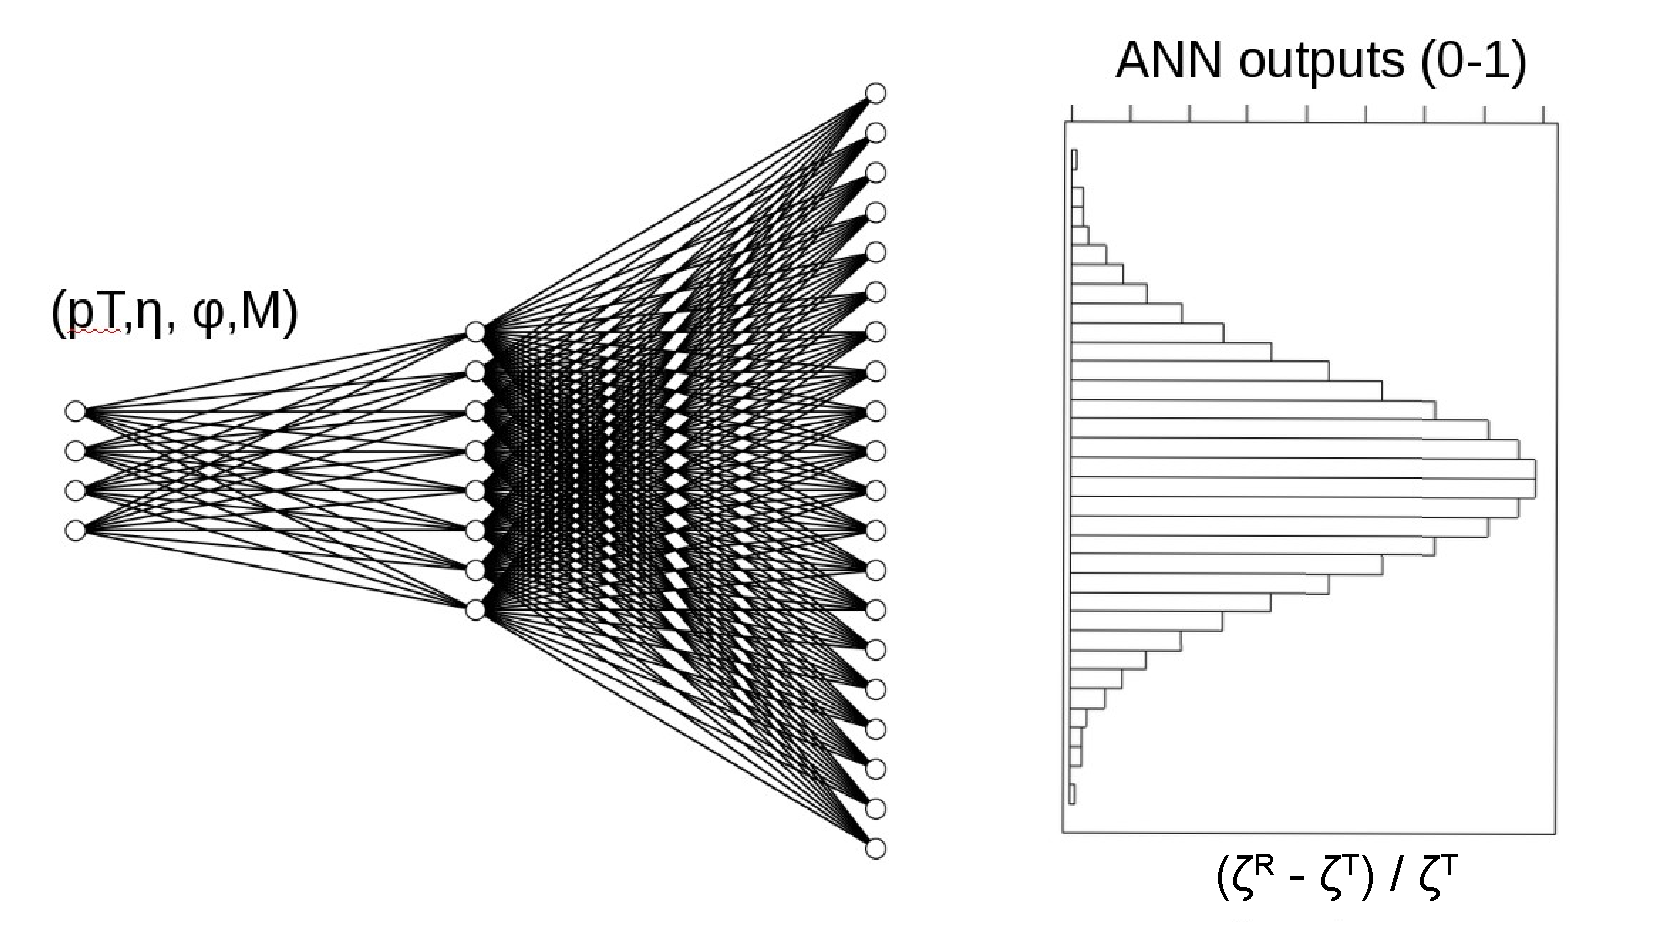
\includegraphics[width=0.8\textwidth]{figures/intro/nn_example.pdf}
  \caption{A schematic representation of the NN architecture for modelling the detector response and affect of reconstruction algorithms on truth-level input variables. The output of this NN is a PDF for the resolution of single variable, e.g. \ptRes.}
  \label{ann_example}
\end{figure}


%%%%%%%%%%%%%%%%%%%%%%%%%%%%%%%%%%%%%%%%%%%%% 
\section{Monte Carlo simulated event samples}
%%%%%%%%%%%%%%%%%%%%%%%%%%%%%%%%%%%%%%%%%%%%% 

Monte Carlo events used for this analysis were produced using the Madgraph generator~\cite{Alwall:2014hca}. The simulated processes are a combination of equal parts top pair production ($t\bar{t}$+jets) and photons produced in association with jets ($\gamma$+jets), which give a high rate of jets in different environments. 
Hadronic jets were reconstructed with the {\sc FastJet} package~\cite{Fastjet} using the anti-$k_t$ algorithm \cite{Cacciari:2008gp} with a distance parameter of 0.4. The detector simulation was performed with the Delphes package with a detector geometry which is similar to the ATLAS geometry. 
The event samples used in this paper, before and after the fast simulation, are available from the HepSim database~\cite{Chekanov:2014fga}. In this paper only the transformation from truth jets (which have truth particle constituents) to reconstructed jets (which calorimeter cell constituent) and only for \pt\ was performed, however the methodology should be object and parameter agnostic. Truth jets which were matched to a reconstructed Delphes jet are used. For the matching criteria the reconstructed jet that has the smallest $\Delta R=\sqrt{\Delta\phi^2+\Delta\eta^2}$, where $\Delta\phi=\phi^{\text{truth}}-\phi^{\text{reco}}$ and $\Delta\eta=\eta^{\text{truth}}-\eta^{\text{reco}}$, with respect to the truth jet is chosen. If this minimum $\Delta R$ is greater than 0.2, the truth jet is discarded. No other requirements are made on truth and reconstructed Delphes jets other than the $\pt>15$ GeV requirement made by Delphes. Only matched jets are used for this study since the aim of the study is to test whether an NN can changes in detector resolution as a function of kinematic properties of the jet (e.g. $\pt$, $\eta$, $\phi$, $m$). 
The final number of training jets used is two million while 500,000 jets were used as a testing sample. The distributions of quantities used as the input for the NN, \pt, $\eta$\, $\phi$, $m$, are shown in Figure~\ref{fig:nnInputsPrescaling}.

\begin{figure}[h]
  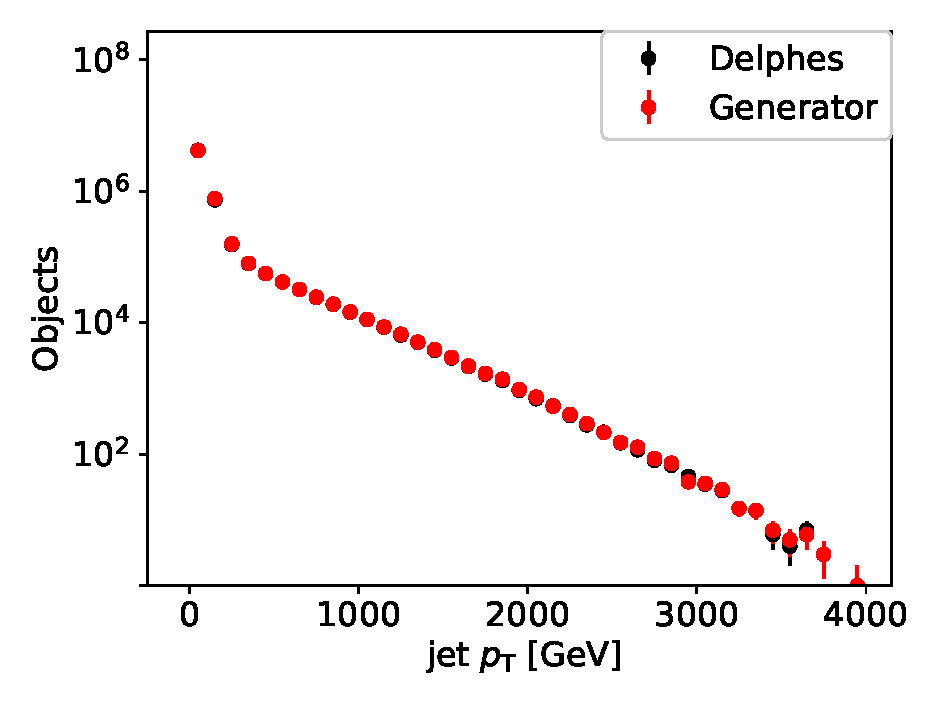
\includegraphics[width=0.48\textwidth]{figures/nn/jet_pT_prescaling_log.eps}
  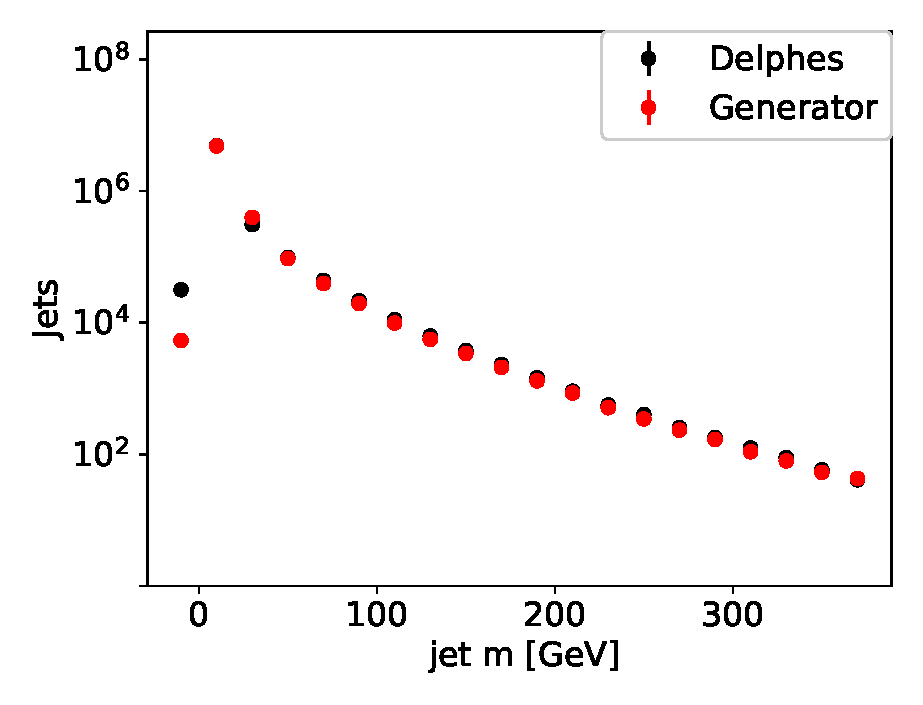
\includegraphics[width=0.48\textwidth]{figures/nn/jet_m_prescaling_log.eps}\\
  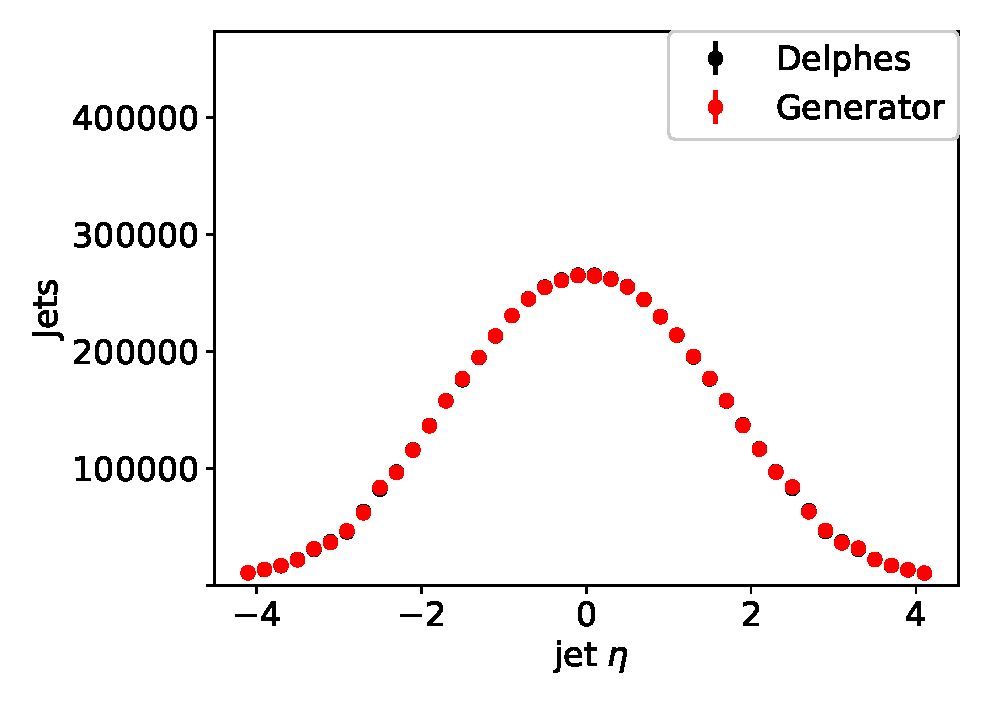
\includegraphics[width=0.48\textwidth]{figures/nn/jet_eta_prescaling.eps}
  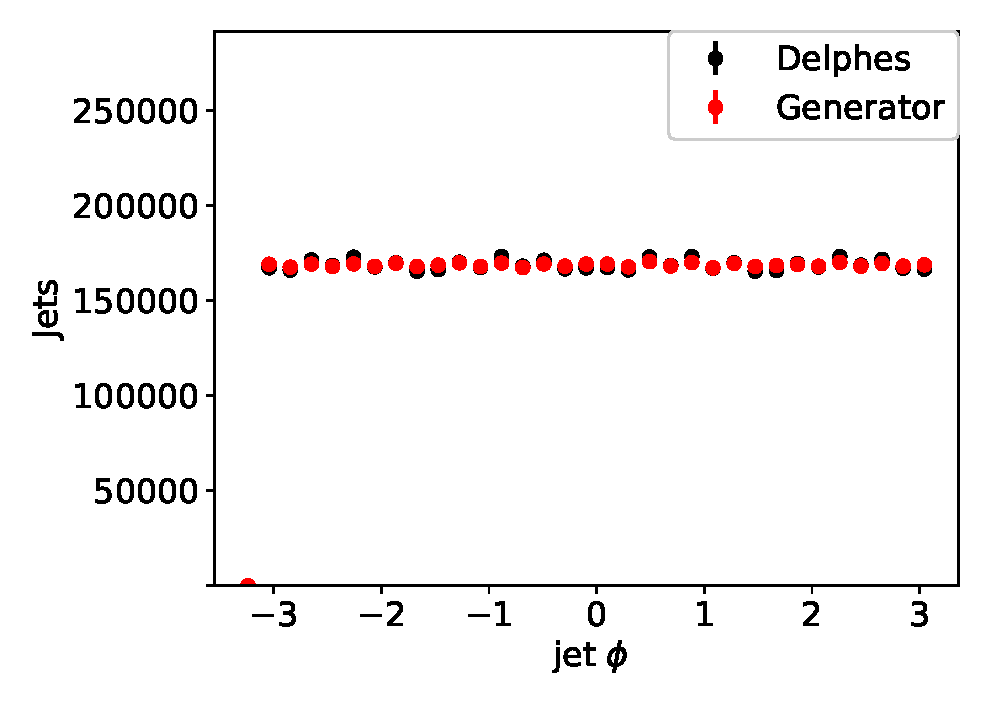
\includegraphics[width=0.48\textwidth]{figures/nn/jet_phi_prescaling.eps}
  \caption{Distributions for input variables for truth (red) and reco quantities (black).}
  \label{fig:nnInputsPrescaling}
\end{figure}

To facilitate gradient descent in all direction of the input variables, the input variables are scaled to be in the range [0,1]. This avoids the \pt\ and the mass from having a disproportional affect on the training of the NNs. The output variable, \ptRes, is also scaled to have values between 0 and 1. Only objects that 
are within the 1$^{\mathrm{st}}$ and 99$^{\mathrm{th}}$ percentile of the \ptRes\ distribution are considered in this study since objects outside this range are typically not used in physics analyses.

\begin{figure}[h]
  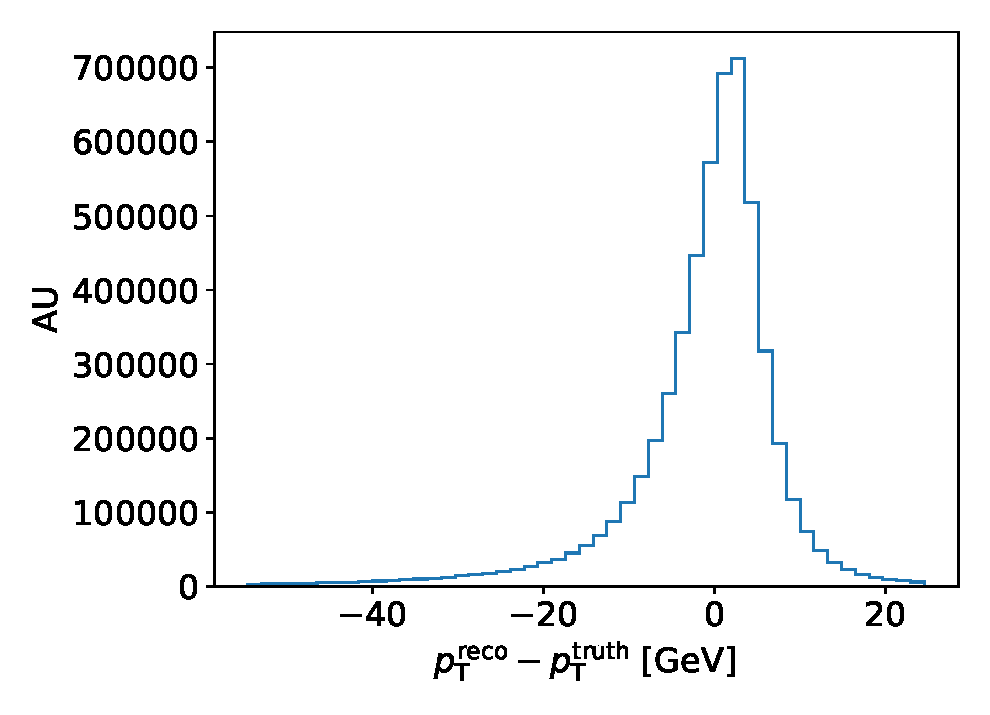
\includegraphics[width=0.48\textwidth]{figures/nn/pTRes_nobounds_prescaling.eps}
  \caption{Relative differences between truth and reco \pt.}
  \label{fig:deltaTarget}
\end{figure}


\section{Neural network structures}

An NN is trained with four input parameters, the scaled \pt, $\eta$, $\phi$, and $m$, and consist of five layers with 100 nodes each and with each node having a rectifier linear unit (ReLu) activation function. The output layer has 400 nodes with a softmax activation function. Finally, the NN is trained over 1000 epochs with batch size 1000 using the Adam~\cite{adam} optimizer with a learning rate of $10^{-4}$. The NN is implemented using Keras~\cite{chollet2015keras} with a TensorFlow~\cite{tensorflow2015-whitepaper} backend.


%%%%%%%%%%%%%%%%%%%%%%%%%%%%%%%%%%%%%%%%%%%%% 
\section{Results}
%%%%%%%%%%%%%%%%%%%%%%%%%%%%%%%%%%%%%%%%%%%%% 

After the NN has been trained to learn the PDF of \ptRes, the resulting learned PDF is compared to the Delphes PDF using the testing sample in Fig.~\ref{fig:PDFComp}a. Good agreement is observed between the Delphes and NN PDFs, showing that the NN has learned the bulk distribution.

\begin{figure}[htb]
  \subfigure[]{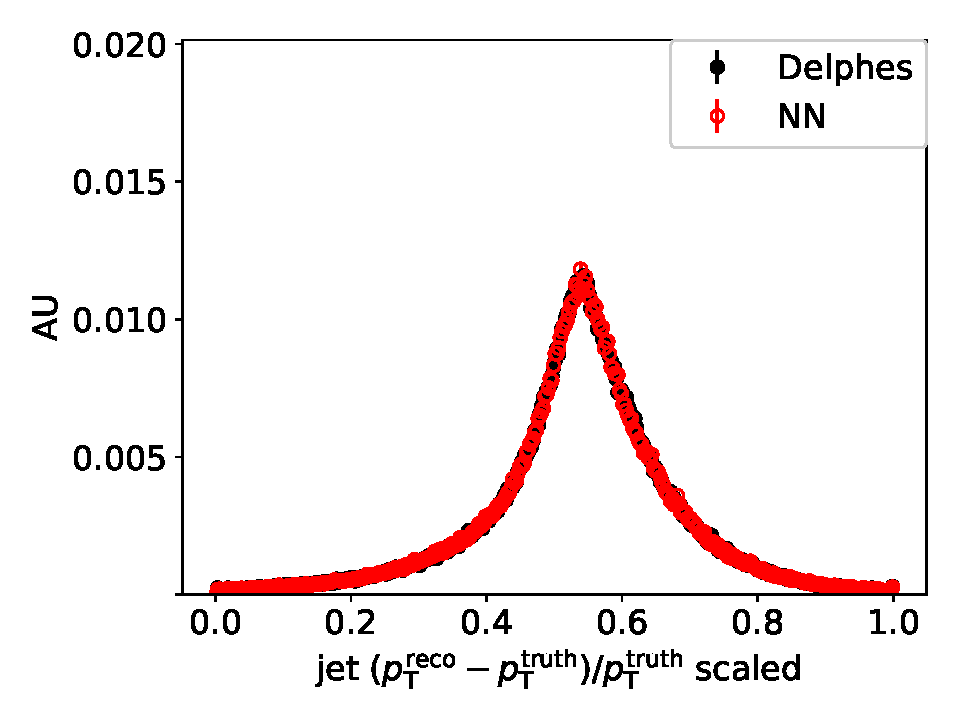
\includegraphics[width=0.48\textwidth]{figures/nn/jet_pTRes_batchSize1000_epochs1000.eps}}
  \subfigure[]{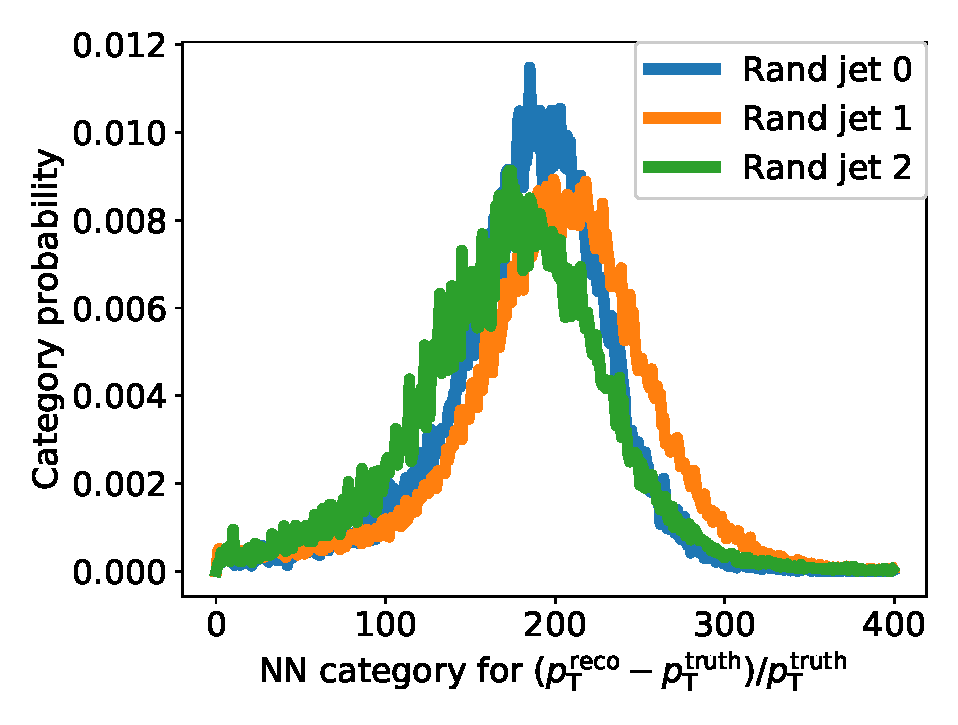
\includegraphics[width=0.48\textwidth]{figures/nn/nnOutput_pT_batchSize1000_epochs1000.eps}}
  \caption{NN-generated jet \ptRes\ compared to reco Delphes jet \ptRes\ (a). NN-generated jet PDFs for three randomly selected truth jets (b).}
  \label{fig:PDFComp}
\end{figure}

The NN predicts a PDF for each jet based on its input parameters (i.e. \pt, $\phi$, $\eta$, and $m$). The PDFs for a set of randomly selected jets are shown in Fig.~\ref{fig:PDFComp}b. These PDFs are then randomly sampled to produce an NN jet that mimics the reco jet. A comparison of the NN-generated and Delphes jet \pt\ distribution for the testing sample is shown in Fig.~\ref{fig:pTNNVsDelphes}. The NN reproduces the jet \pt\ distribution of Delphes within 5\% for reconstructed jets with $\pt>20$ GeV. 


\begin{figure}[htb]
  \subfigure[]{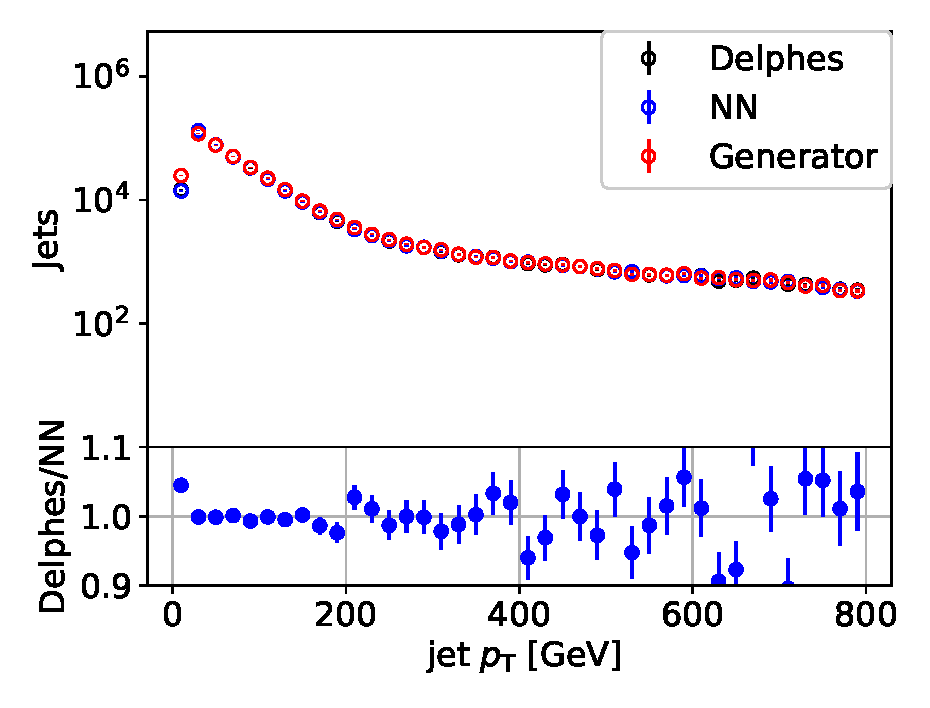
\includegraphics[width=0.42\textwidth]{figures/nn/jet_pT_genVsReco_origScale_test_batchSize1000_epochs1000_log.eps}}
  \subfigure[]{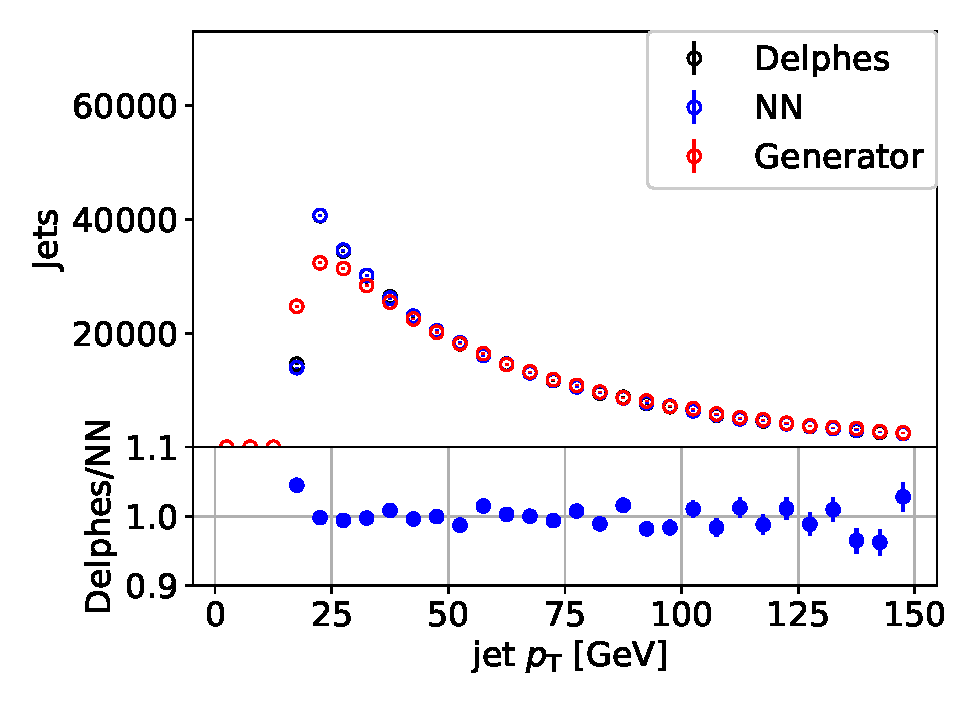
\includegraphics[width=0.48\textwidth]{figures/nn/jet_pT_genVsReco_origScale_zoom_test_batchSize1000_epochs1000.eps}}
  \caption{Delphes and NN-generated jet \pt\ disitributions for a wide (a) and narrow (b) \pt\ range.}
  \label{fig:pTNNVsDelphes}
\end{figure}

To test whether the NN learned correlations between input parameters and the \pt\ resolution, the jets were divided into central ($|\eta|<3.2$) and forward ($|\eta|>3.2$) jets. The \pt\ resolution is then compared between the two regions for both the Delphes jets as well as the NN-generated jets. These two regions in the detector simulation have different calorimeter resolutions which results in different jet \pt\ resolutions and thus the \pt\ resolution is correlated with $|\eta|$. The resulting resolutions for both regions are shown in Fig.~\ref{fig:nnRes} using the training sample. The training sample was chosen for this comparison because forward jets make up a small subsample of all jets, as can be seen in Fig.~\ref{fig:nnInputsPrescaling}. Several batch-size and number-of-epoch combinations were used in an attempt to optimize the sensitivity to a small subsample (the forward jets) of the training sample. The number of backpropagations ($N_{bp}$) were held constant by keeping the ratio of the number of epochs ($N_e$) and batch size ($N_b$) constant since $N_{bp}=\frac{N_t}{N_b}N_e$ where $N_t$ is the number of training jets. Batch size and number of epochs of 5, 10, 20, 100, 200, 1000 were tested resulting in similar performance of the NN in both the central and forward region.

\begin{figure}[htb]
  \includegraphics[width=0.48\textwidth]{figures/nn/jet_pTResEta_batchSize1000_epochs1000.eps}
  \caption{Jet \pt\ resolution for the training sample for both the central and forward region. }
  \label{fig:nnRes}
\end{figure}

To test whether what the NN learned is sample independent we applied the NN to a top pair production in association with a $W$ boson ($t\bar{t}+W$) sample which contained 900,000 jets. This sample is expected to have higher jet multiplicities per event. The \pt\ distributions over two \pt\ ranges are shown in Fig.~\ref{fig:pTNNVsDelphes_ttW} while the comparison between the central and forward jet \pt\ resolutions can be seen in Fig.~\ref{fig:nnRes_ttW}. The agreement in Fig.~\ref{fig:pTNNVsDelphes_ttW} is good for jets with $\pt<200$ GeV but a mismodeling trend appears at \pt s greater than 200 GeV. We expect this to be due high \pt\ $b$-jets which are not as prevalent in the training set where the high \pt\ jets mainly come from the $\gamma$+jets sample which is produced to have a flattened \pt\ spectrum. For future studies and refinements one could add truth $b$-quark information to help improve the modelling of these types of jets.  


\begin{figure}[htb]
  \subfigure[]{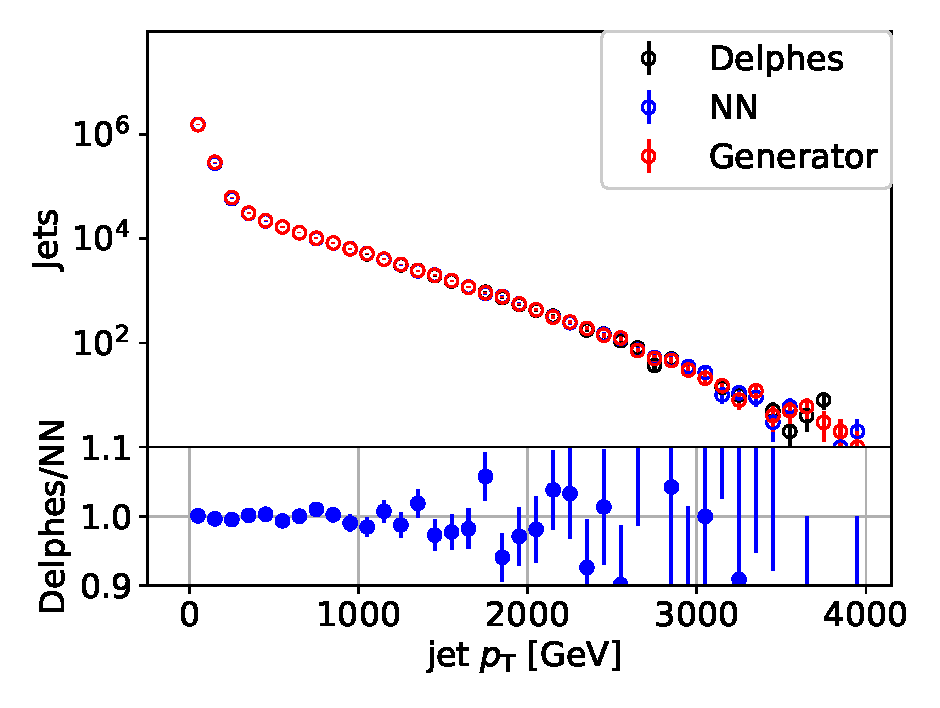
\includegraphics[width=0.42\textwidth]{figures/nn/ttW/jet_pT_genVsReco_origScale_train_batchSize1000_epochs1000_log.eps}}
  \subfigure[]{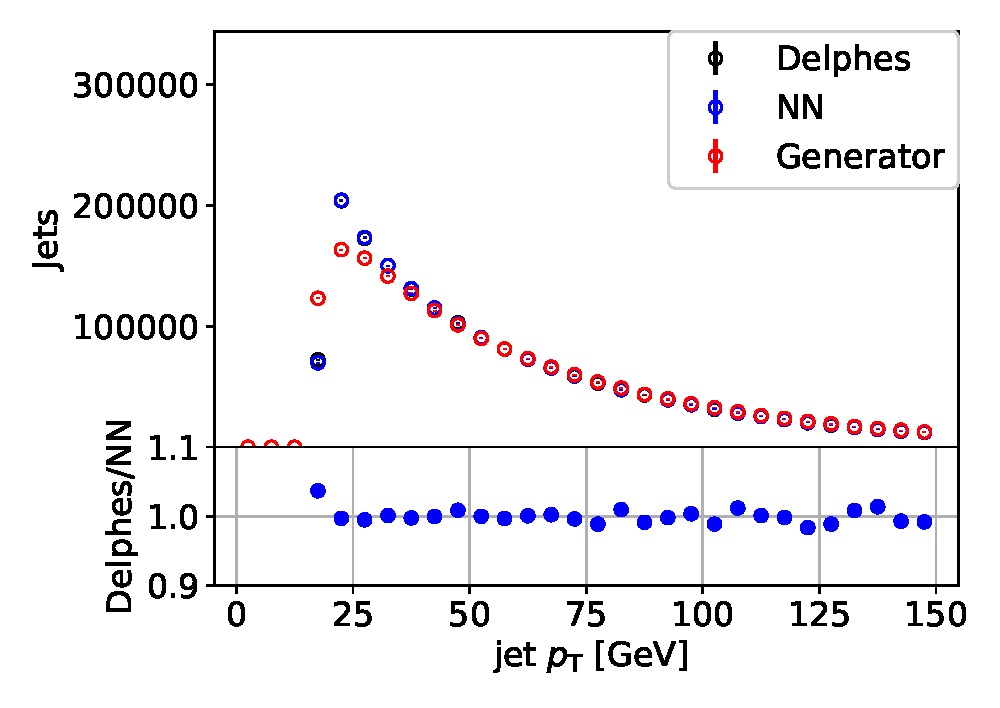
\includegraphics[width=0.48\textwidth]{figures/nn/ttW/jet_pT_genVsReco_origScale_zoom_train_batchSize1000_epochs1000.eps}}
  \caption{Delphes and NN-generated jet \pt\ disitributions for a wide (a) and narrow (b) \pt\ range for jets originating from $t\bar{t}+W$ production.}
  \label{fig:pTNNVsDelphes_ttW}
\end{figure}


\begin{figure}[htb]
  \includegraphics[width=0.48\textwidth]{figures/nn/ttW/jet_pTResEta_batchSize1000_epochs1000.eps}
  \caption{Jet \pt\ resolution for the training sample for both the central and forward region for jets originating from $t\bar{t}+W$ production.}
  \label{fig:nnRes_ttW}
\end{figure}

% \section{Hyperparameter optimization}
% In order to acquire the optimal performance with an NN with a minimal amount of parameters, a genetic algorithm (GA) was used to optimize the NN hyperparameters. Hyper parametrization, that is, the determination of the optimal parameters associated with a complex NN (number of layers, number of neurons on each layer, choice of the learning rate, mini-batch size), is a challenging optimization problem in a high dimensionality space, especially for nonlinear NNs. Ultimately, the range of hyperparameter values that must be explored grows dramatically as the complexity of the deep NN increases. To address this challenge, we have used a GA, which is an evolutionary algorithm that mimics the process of natural selection. Previously successful applications of the GA in similar contexts include the determination of the parameters of a complex force field~\cite{doi:10.1021/acs.jctc.7b00521,doi:10.1021/acs.jctc.6b00432}. 
% A flowchart of the ML/GA optimization protocol is depicted in Fig.~\ref{fig:hyperFlow}. The optimization starts with a set of parent parameters, which is defined as the population. For hyperparameter optimization of the NN, the parents sets are number of layers, number of neurons on each layer, choice of the learning rate or mini-batch size. Some of the individuals in this population present a better fit, which in the context of NNs means a higher value for the accuracy of the network. Fit parents survive and are allowed to mate, which is accomplished by crossing patterns with other fit individuals. During crossover, random mutations in the genes are also allowed, to a certain degree, to avoid a stagnant gene pool and a better sampling of the parameters space. The offspring individuals form the next generation of parents and this process continues until some predefined criteria are met. Sets of parameters are then ranked in ascending order. After the ranking, a nonlinear roulette wheel selection~\cite{DBLP:journals/corr/abs-1109-3627} was performed to select the best 60\% members, that is, the ones with lowest values of accuracy, which were then subjected to genetic operations: mutation and crossover with a 3\% crossover rate. These mutations introduce sufficient diversity into the population, and the nonlinear selection scheme helps to avoid premature convergence of the ML/GA run. After the genetic operations, both the parent and offspring sets of parameters are ranked by their value of accuracy. The best hyperparameter sets are then chosen to constitute the next generation. Such an optimization routine ensures that only satisfactory hyperparameter sets survive after each generation; upon repeating this workflow for sufficient generations and sampling viable regions in the parameter space, we performed three separate ML/GA runs starting with different random populations. From each of the converged ML/GA run, we chose the final hyperparameter set corresponding the highest value of accuracy. 


% \begin{figure}[htb]
%   \subfigure[]{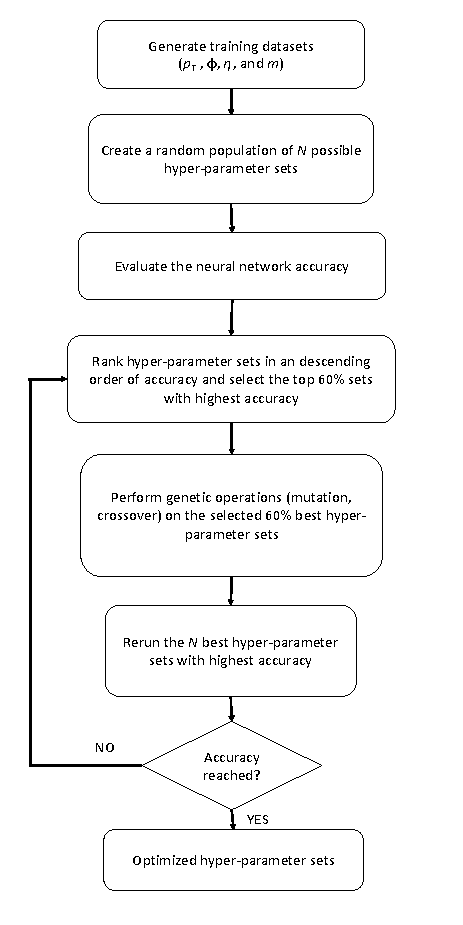
\includegraphics[width=0.48\textwidth]{figures/hyperparam.pdf}}
%   \caption{Flow chart of the hyperparameter optimization used to optimize the resolution NN.}
%   \label{fig:hyperFlow}
% \end{figure}

\section{Conclusion}

We have shown that a truth-level quantity can be transformed to a reconstruction-level quantity using a multi-categorizing NN. The NN learned the truth-to-reconstruction transformation without requiring manual binning to capture the differences in resolutions of particular subsamples (central and forward jets). To ensure that this method produces realistic results, the training data needs to be carefully chosen to properly represent objects that one wants to transforms (as was shown in when the NN is applied to the $t\bar{t} W$). Additional improvements could be made by including more information about the objects (e.g. whether a $b$-quark is present in a jet, kinematic information from other objects in the event) making this method more robust. This method should be easily extendable to additional reconstructed quantities and could be used to model the ATLAS and CMS detector. The method described in this paper thus allows for automated detector parameterization which can facilitate phenomological studies, efficient truth event selection, and upgrade studies.

\section*{Acknowledgments}
The submitted manuscript has been created by UChicago Argonne, LLC, Operator of Argonne National Laboratory (“Argonne”). Argonne, a U.S.  Department of Energy Office of Science laboratory, is operated under Contract No. DE-AC02-06CH11357. The U.S. Government retains for itself, 
and others acting on its behalf, a paid-up nonexclusive, irrevocable worldwide license in said article to reproduce, prepare derivative works, distribute copies to the public, and perform publicly and display publicly, by or on behalf of the Government.  The Department of Energy will provide public access to these results of federally sponsored research in accordance with the 
DOE Public Access Plan. \url{http://energy.gov/downloads/doe-public-access-plan}. Argonne National Laboratory’s work was funded by the U.S. Department of Energy, Office of High Energy Physics under contract DE-AC02-06CH11357. 



%%%%%%%%%%%%%%%%%%%%%% references %%%%%%%%%%%%%%%%%%%%%%%%%%%%%%
% \clearpage
\bibliographystyle{unsrt}   % this means that the order of references
% is dtermined by the order in which the
% \cite and \nocite commands appear
\bibliography{main}  % list here all the bibliographies that
% you need. 


\end{document}